\documentclass[
  11pt,
  letterpaper,
  % addpoints,
  answers
]{exam}

\usepackage{../tarea}

\begin{document}
\begin{minipage}{0.42\textwidth}
    
\includegraphics[width=\textwidth]{../fcfm_die}
\end{minipage}
\begin{minipage}{0.53\textwidth}
\begin{center} 
\large\textbf{Clases Particulares} \\
\normalsize Prof.~Gonzalo Narváez.
\end{center}
\end{minipage}

\vspace{0.5cm}
\noindent
\begin{questions}

\question[10]{Sea una línea de transmisión visto en la \cref{fig:lt} de impedancia característica $Z_0 = 50\,\Omega$, se le adiciona una linea de transmisión de longitud $l = 5\lambda/12$ en circuito abierto.}
\begin{parts}
  \part[2]{Calcule la impedancia $Z_{ca}$ del circuito.}
  \part[2]{Calcule la impedancia equivalente en la linea de transmisión.}
  \part[4]{Determine las distancias $l$ y $l_s$ necesarias para adaptar la línea de transmisión utilizando la Carta de Smith, implementando un stub en cortocircuito y otro en circuito abierto.}
  \part[2]{Explique detalladamente el proceso de adaptación.}
\end{parts}

\begin{figure}[ht]
    \centering
    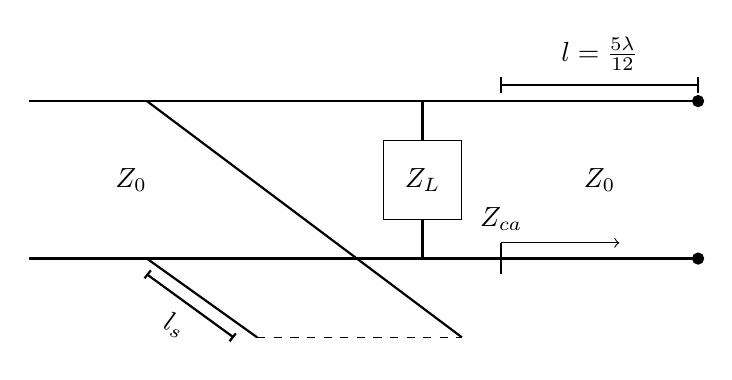
\begin{tikzpicture}
      % Línea de transmisión
      \draw[thick] (-4,1) -- (4.5,1);  % Línea superior
      \draw[thick] (-4,-1) -- (4.5,-1); % Línea inferior
      \draw[thick] (2,1.2) -- (4.5,1.2); % Línea derecha


      %stub
      \draw[thick] (-2.5,1) -- (1.5,-2); % Línea vertical
      \draw[thick] (-2.5,-1) -- (-1.1,-2); % Línea vertical
      %\draw[thick] (-0.9,-2) -- (1,-2); % Línea izquierda

      %distancia ls

      \draw[thick] (-2.5,-1.2) -- (-1.4,-2); % Línea vertical
      \draw[thick] (-2.53,-1.25) -- (-2.45,-1.15); % Línea izquierda
      \draw[thick] (-1.45,-2.05) -- (-1.37,-1.95); % Línea derecha
      \node[rotate=-22] at (-2.15,-1.85) {$l_s$}; % Rotación
      \draw[dashed] (-1.1,-2) -- (1.5,-2); % Línea punteada


      % flecha longitud de onda
      \draw[thick] (2,1.1) -- (2,1.3); % Línea izquierda
      \draw[thick] (4.5,1.1) -- (4.5,1.3); % Línea izquierda

      

      \draw[thick] (1,1) -- (1,0.5); % Línea vertical
      \draw[thick] (1,-1) -- (1,-0.5); % Línea vertical
      \draw (1.5,0.5) rectangle (0.5,-0.5); % Rectángulo
      \node at (1,0) {$Z_L$}; % Etiqueta dentro del rectángulo

      % flecha impedancia circuito abierto
      \draw[thick] (2,-1.2) -- (2,-0.8); % Línea derecha
      \draw[->] (2,-0.8) -- (3.5,-0.8);

      % circuito abierto 
      \filldraw[black] (4.5,-1) circle (2pt);
      \filldraw[black] (4.5,1) circle (2pt);

      \node at (-2.7,0) {$Z_0$};
      \node at (3.25,0) {$Z_0$};
      \node at (3.25,1.6) {$l = \frac{5\lambda}{12}$};
      \node at (2,-0.5) {$Z_{ca}$};

    \end{tikzpicture}
    \caption{Linea de transmisión en circuito abierto.}
    \label{fig:lt}
  \end{figure}


\begin{solution}
\begin{parts}
\part{La impedancia $Z_{ca}$ del circuito se calculará con la formula $Z_{in}$ para la cual se tiene que $Z_L = \infty$ y $Z_0 = 50\,\Omega$.}

\begin{align}
  Z_{ca} &=\frac{Z_{0} (Z_{l}+ jZ_{0}\tan(\beta l))}{(Z_{0}+jZ_{l}\tan(\beta l))}\\
  &= Z_{0} \frac{\del{ 1 + \frac{jZ_{0}\tan(\beta l)}{Z_{l}}}}{\del{(\frac{Z_{0}}{Z_{l}} + j\tan(\beta l)}}\\
  &= \frac{-jZ_{0}}{\tan\del{\frac{2\pi}{\lambda} \frac{5\lambda}{12\pi}}}\\
  &= \frac{-jZ_{0}}{\tan\del{\frac{5\pi}{6}}}\\
  &= \frac{j \sqrt{3}Z_{0}}{3}
\end{align}
\part{La impedancia equivalente en la linea de transmisión será la impedancia de circuito abierto en paralelo con la impedancia de la carga $Z_{eq} = Z_{ca}//Z_{l}$.}





\end{parts}
\end{solution}


\end{questions}
\end{document}
